\documentclass{report}
\usepackage[latin1]{inputenc}
\usepackage[T1]{fontenc}
\usepackage{amsmath}
\usepackage{amssymb}
\usepackage[top=5cm, bottom=5cm, left=3cm, right=3cm]{geometry}
\pagestyle{headings}
\usepackage{lmodern}
\usepackage{enumitem}
\usepackage{float, graphicx}
\usepackage{hyperref}
\DeclareMathOperator{\argmax}{argmax}

\title{\textbf{Stochastic Lab Course 1}}
\author{Khwam Tabougua Trevor}
\date{October 2018}
\begin{document}
	
\maketitle

\chapter*{Introduction}

The "Stochastic Lab course I" is an Introductory Course for
statistics and stochastics applications with R programming language. The course lasted for two weeks in September 2018. The report contains results, interpretations and figures from the ten exercises that had to be solved. Along with this report, there is also the R codes, which are helpful to understand the results.

\tableofcontents
\chapter{Simpson's Paradox}
Simpson's paradox, or the Yule-Simpson effect, is a phenomenon in probability and statistics, in which a trend appears in several different groups of data but disappears or reverses when these groups are combined. First mentioned by Karl Pearson (1899) and Udny Yule (1903), it is a paradox where it is possible to draw two opposite conclusions from the same data depending on how things are divided up, and statistics alone cannot help us solve it - we have to go outside statistics and understand the causality of the situation at hand.

\section{Introduction and description of the problem}
To explain Simpson's paradox we start with a hypothetical example from the following website: \href{https://www3.nd.edu/~busiforc/handouts/Other%20Articles/simponsparadox.html}{Simpson's Paradox} . During a particular summer, an experiment was conducted to find out the preference between two types of beverages: soda and lemonade. The data was drawn from two locations: city and rural. In each location, the gender and the choice of drinks were collected. The results are summarized as follows:

\begin{center}
	\begin{tabular}{|c|c|c|c|c|c|c|}
		\hline
		location & gender & lemonade & soda & total & \% preferring lemonade & odds ratio\\ 
		\hline
		city & female & 150 & 300 & 450 & 24.9\% & 1.10\\
		\hline
		     & male & 300 & 660 & 960 & 23.1\% &       \\
		\hline
		rural & female & 285 & 860 & 1145 & 33.3\% & 1.10\\
		\hline
		      & male & 30 & 100 & 130 & 31.3\% &       \\
		\hline
	\end{tabular}
\end{center}

The odds ratio given that location = city is about 1.1, showing that females are about 10\% more likely to drink lemonade than males. Because the conditional odds ratio given that location = rural is also 1.1, the same conclusion can be drawn.\\
Next, combine the results from both locations and form the following 2 by 2 contingency table:

\begin{center}
	\begin{tabular}{|c|c|c|c|c|c|}
		\hline
		gender & lemonade & soda & total & \% preferring lemonade & odds ratio \\ 
		\hline
		female & 435 & 1160 & 1595 & 27.3\% & 0.86 \\
		\hline
		male & 330 & 760 & 1090 & 30.3\% &         \\
		\hline
	\end{tabular}
\end{center}

The odds ratio of 0.86 shows that females are about 14\% less likely to drink lemonade than males, rather than 10\% more likely as was shown earlier! This is an example of Simpson's paradox.\\
In the following exercise, we wxill make use of some graphical tools such as barplots and pie charts to illustrate the paradox.

\section{Exercise}
In this exercise, we use the following data from Moore, D.S. (2003) \textit{The basic practice of statistics} which contains number of delayed and on time flights for two airlines at five US airports in one month.

\begin{center}
	\begin{tabular}{|c|cc|cc|}
		\hline
		         & \multicolumn{2}{c|}{Alaska Airlines} & \multicolumn{2}{c|}{America West}\\
		\hline
		         & On time & Delayed & On time & Delayed\\ 
		\hline
		 Los Angeles & 497 & 62 & 694 & 117\\
		\hline
    	 Phoenix & 221 & 12 & 4840 & 415\\
    	\hline
	     San Diego & 212 & 20 & 383 & 65\\
	    \hline
	     San Francisco & 503 & 102 & 320 & 129\\
	    \hline
	     Seattle & 1841 & 305 & 201 & 61 \\
		\hline
	\end{tabular}
\end{center}

\begin{enumerate}[label=(\alph*)]
	\item Cf. R code
	
	\item When we look at the following plots, we can say that barplot is more suitable for
	this type of comparison. Actually, if we have more variable into our data, using a pie chart will be very difficult for the human eye to estimate the magnitude of angles, thus making visualization not very clear.
	
	\begin{figure}[H]
		\begin{center}
			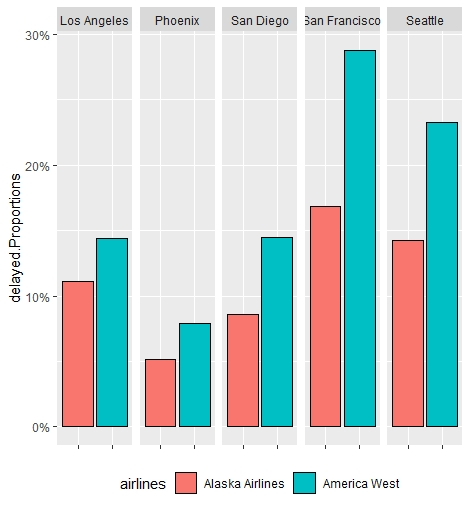
\includegraphics{1_plot_1}
		\end{center}
		\caption{Histogram of the percentage of airlines' delayed flights in each city}
	\end{figure}
	
	\begin{figure}[H]
		\begin{center}
			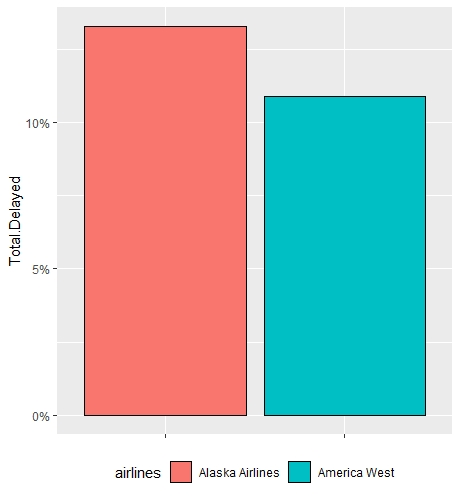
\includegraphics{1_plot_2}
		\end{center}
		\caption{Histogram of the total percentage of airlines' delayed flights}
	\end{figure}
	
	\begin{figure}[H]
		\begin{center}
			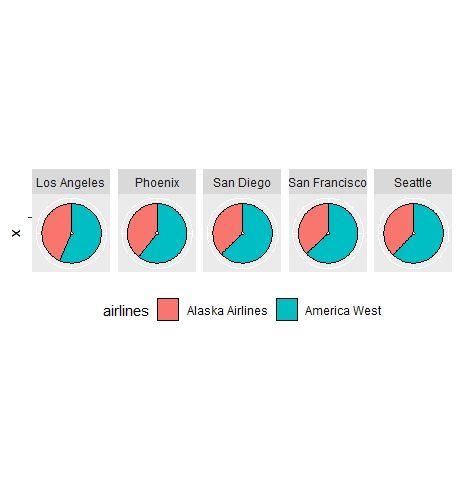
\includegraphics{1_plot_3}
		\end{center}
		\caption{Piechart of the percentage of airlines' delayed flights in each city}
	\end{figure}

\begin{figure}[H]
	\begin{center}
		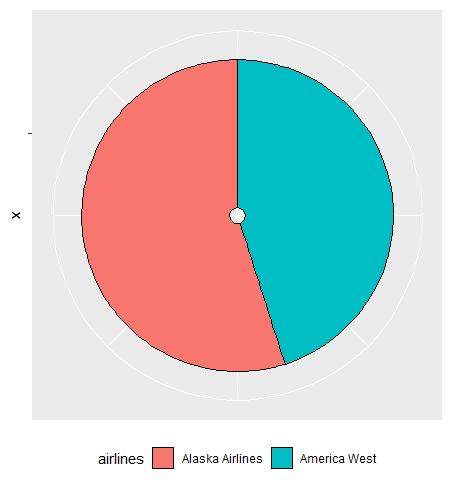
\includegraphics{1_plot_4}
	\end{center}
	\caption{Piechart of the total percentage of airlines' delayed flights}
\end{figure}

\item Plots in Figure 1.1 and Figure 1.3 clearly shows how in each city, the percentage of delayed flights for Alaska Airlines is less than the one of America West. Therefor one would expect to have the same result when looking at the delayed flights of these airlines in the all the five cities. According to Figure 1.2 and Figure 1.4, this is not the case, since it illustrates how that percentage for Alaska Airlines is larger than the one of America West: this is the Simpson's paradox.

\end{enumerate}

\chapter{Descriptive statistics }
Descriptive statistics are used to describe the basic features of the data in a study. They provide simple summaries about the sample and the measures. Together with simple graphics analysis, they form the basis of virtually every quantitative analysis of data.

\section{Introduction and description of the problem}
First of all, we have the summary statistics, which are used to summarize a set of observations, in order to communicate the largest amount of information as simply as possible. We commonly try to describe the observations with the mean, the variance, the $\alpha$-quantile, the median, and the IQR (Interquartile range). Furthermore, there are histograms, boxplots and Q-Q-plots to illustrate these key figures and the quantiles in general. Note that a histogram is constructed by first deciding on a set of classes, or bins, which partition the real line into a set of boxes into which the data values fall. Then vertical bars are drawn over the bins with height proportional to the number of observations that fell into the bin.

\section{Exercise}
In this exercise, we are using the dataset from \href{https://archive.ics.uci.edu/ml/datasets/Wine+Quality}{UCI Machine learning repository} on the white wine quality.

\begin{enumerate}[label=(\alph*)]
	\item Cf. R code. After loading the data into R, a new binary variable good which is 1
	if quality > 5 and 0 otherwise, is added to the data frame. We would like to compare \textbf{volatile.acidity} and \textbf{residual.sugar} for good and bad wines.
	
	\item At first, we consider the variable \textbf{residual.sugar}.
	\item[�] Here, we plot histograms of \textbf{residual.sugar} for good and bad wines. We have to note that when using histograms in R, the data is grouped into 30 bins. This may be too fine or too coarse for our data. Here, we are using Sturges' formula, Scott's choice, and FreedmanDiaconis' choice to specify the bin's width. In Figure 2.1, we notice that the histogram using Sturges' formula is more accurate than the two others, when we compare them to the histogram with no bin width. Therefor Sturges' formula is adequate for our data. It is the same result we have in Figure 2.2. Furthermore, the distributions of Good and Bad white wine and Bad white is highly skewed to the right. We have evidence against the assumption that their distributions is the normal one.
	
	\begin{figure}[H]
		\begin{center}
			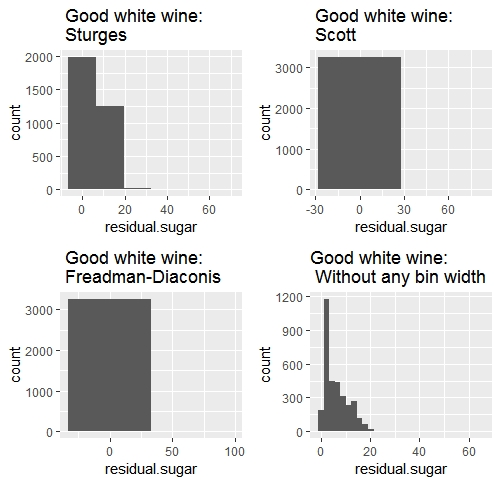
\includegraphics{2_plot_1}
		\end{center}
		\caption{Histograms of residual.sugar for good wines with different bin width methods (available in R) and without}
	\end{figure}
	
	\begin{figure}[H]
		\begin{center}
			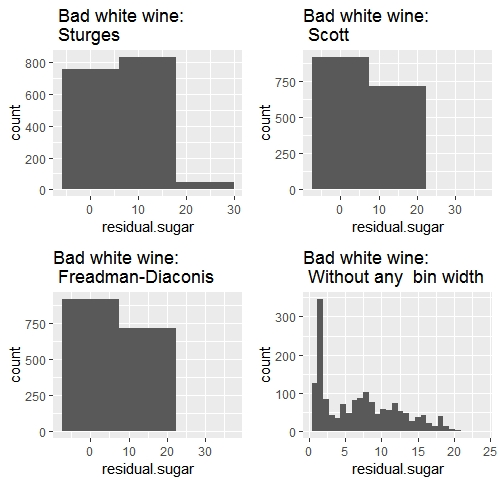
\includegraphics{2_plot_2}
		\end{center}
		\caption{Histograms of residual.sugar for bad wines with different bin width methods (available in R) and without}
	\end{figure}
     
     \item[�] In the table below, we have the summary statistics for both wine groups. We have different mean and median for both groups, which is a confirmation that both groups are not symmetric. Furthermore both groups have approximately the same minimum, but Good wine have a maximum way larger than the one of Bad wine. On the other hand, the interquartile of Good wine is less than the one of Bad wine. Therefor, we can say that data are more spread in the Bad wine group than in the Good wine, and that there is/are one/some outliner(s) in the Good wine group.
     
     \begin{center}
     	\begin{tabular}{|c|c|c|c|c|c|c|}
     		\hline
     		residual.sugar & mean & median & standard deviation & IQR & minimum & maximum \\ 
     		\hline
     		Good wine & 6.057658 & 4.750 & 4.929353 & 7.400 & 0.7 & 65.8 \\
     		\hline
     		Bad wine & 7.054451 & 6.625 & 5.283594 & 9.325 & 0.6 & 23.5 \\
     		\hline
     	\end{tabular}
     \end{center}
     
     \item [�] After generating the boxplots for both samples in Figure 2.3, we can observe that there are four asterisks above the Good wine's boxplot, meaning that there are four outliers in that group.
     
     \begin{figure}[H]
     	\begin{center}
     		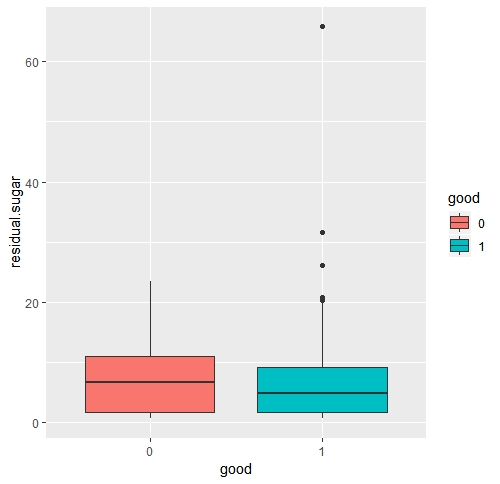
\includegraphics{2_plot_3}
     	\end{center}
     	\caption{Boxplots for both samples}
     \end{figure}
     
     \item[�] In Figure 2.4, we have the QQ-plot to compare the two groups. We can observe that points are slightly above the identity line, and we know that there some outliners in the Good wine group. Therefor we can suggest that if those outliners are removed, we will have all the points aound the identity line. Thus, we can say that the two groups share the same distribution. 
     
     \begin{figure}[H]
     	\begin{center}
     		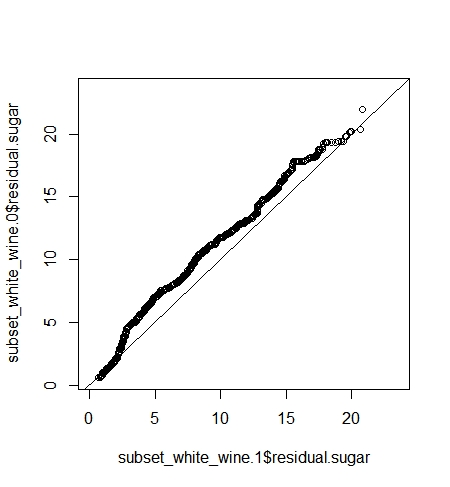
\includegraphics{2_plot_4}
     	\end{center}
     	\caption{QQ-plot to compare the two groups }
     \end{figure}
     
     \item[�] In Figure 2.5, we have the emmpirical distribution functions of both groups. Despite a slight difference on the incresing part of the curves, we can say that the two groups have distributions that are quite similar.
     
     \begin{figure}[H]
     	\begin{center}
     		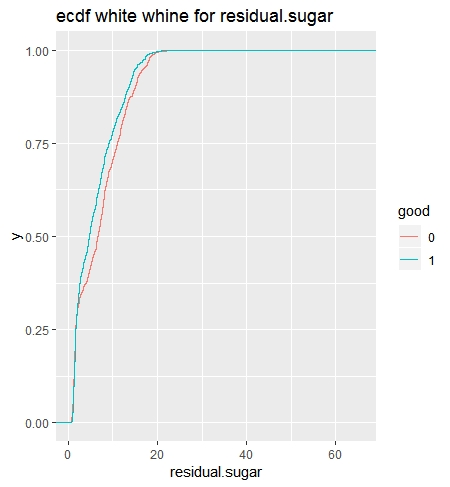
\includegraphics{2_plot_5}
     	\end{center}
     	\caption{Empirical distribution functions of both groups }
     \end{figure}
     
     \item Now we repeat the previous tasks with \textbf{volatile.acidity} for good and bad wines.
     
     \item[�] Here, we plot histograms of \textbf{volatile.acidity} for good and bad wines. In Figures 2.6 and 2.7, we notice that the histograms using bin width formula have the same rectangle shape, Therefor it would best to use the histogram without any bin width. Furthermore, the distributions of Good and Bad white wine and Bad white is highly skewed to the right. We have evidence against the assumption that their distributions is the normal one.
     
     \begin{figure}[H]
     	\begin{center}
     		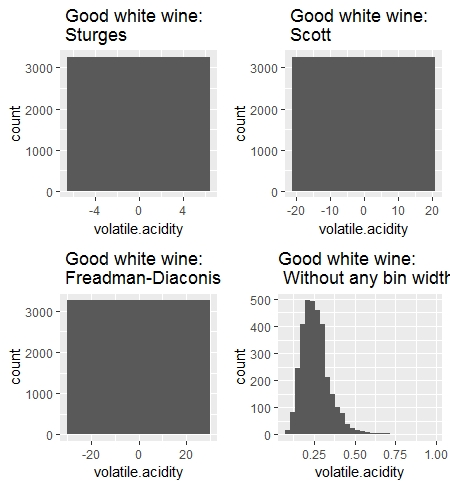
\includegraphics{2_plot_6}
     	\end{center}
     	\caption{Histograms of volatile.acidity for good wines with different bin width methods (available in R) and without}
     \end{figure}
     
     \begin{figure}[H]
     	\begin{center}
     		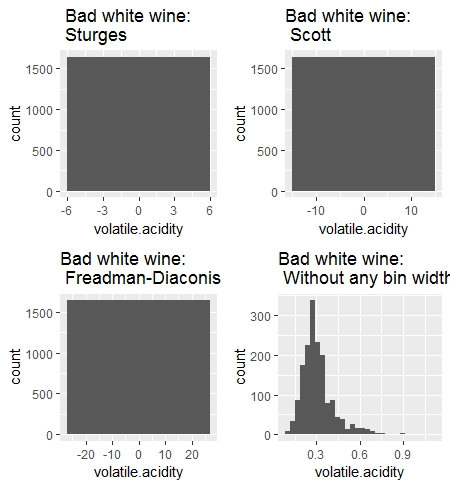
\includegraphics{2_plot_7}
     	\end{center}
     	\caption{Histograms of volatile.acidity for bad wines with different bin width methods (available in R) and without}
     \end{figure}
     
     \item[�] In the table below, we have the summary statistics for both wine groups. We have different mean and median for both groups, which is a confirmation that both groups are not symmetric. Furthermore both groups have approximately the same minimum, but Good wine have a maximum way larger than the one of Bad wine. On the other hand, the interquartile of Good wine is way less than the one of Bad wine. Therefor, we can say that the data contains some outliers in both groups.
     
     \begin{center}
     	\begin{tabular}{|c|c|c|c|c|c|c|}
     		\hline
     		volatile.acidity & mean & median & standard deviation & IQR & minimum & maximum \\ 
     		\hline
     		Good wine & 0.2621209 & 0.250 & 0.090136 & 0.110 & 0.08 & 65.8 \\
     		\hline
     		Bad wine & 7.0544512 & 6.625 & 5.283594 & 9.325 & 0.10 & 1.1 \\
     		\hline
     	\end{tabular}
     \end{center}
     
     \item [�] After generating the boxplots for both samples in Figure 2.8, we can observe that there are some asterisks above the boxplots, meaning that there are many outliers in in both groups.
     
     \begin{figure}[H]
     	\begin{center}
     		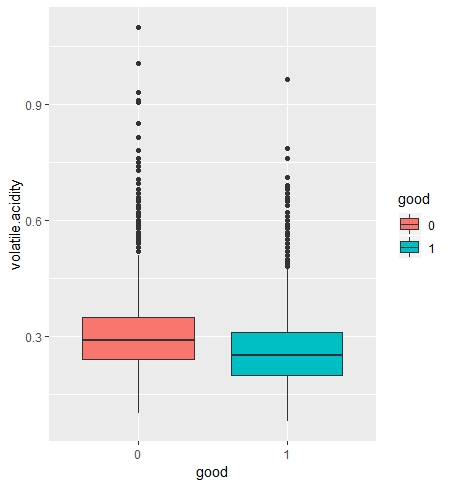
\includegraphics{2_plot_8}
     	\end{center}
     	\caption{Boxplots for both samples}
     \end{figure}
     
     \item[�] In Figure 2.9, we have the QQ-plot to compare the two groups. We can observe that points are slightly moving away the identity line. Therefor we can suggest that both groups do not have the same distribution.
     
     \begin{figure}[H]
     	\begin{center}
     		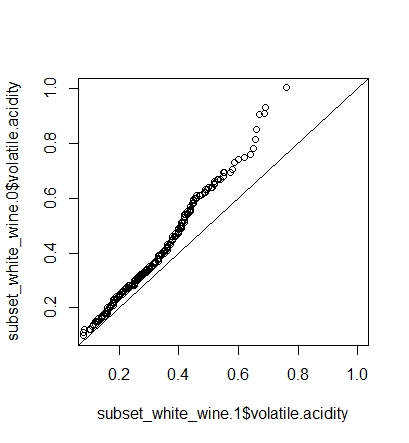
\includegraphics{2_plot_9}
     	\end{center}
     	\caption{QQ-plot to compare the two groups }
     \end{figure}
     
     \item[�] In Figure 2.10, we have the emmpirical distribution functions of both groups. we can notice that we two different curves. Thus, the two groups do not follow the same distribution.
     
     \begin{figure}[H]
     	\begin{center}
     		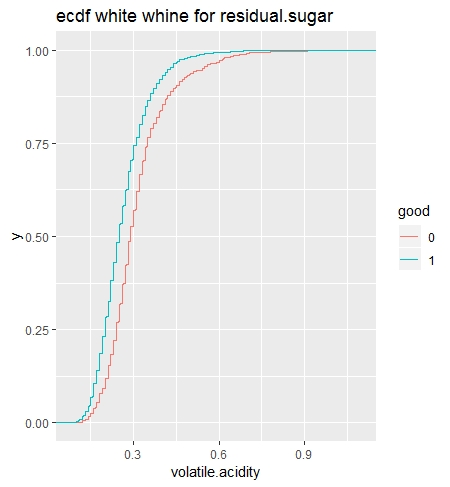
\includegraphics{2_plot_10}
     	\end{center}
     	\caption{Empirical distribution functions of both groups }
     \end{figure}
     
	
\end{enumerate}

\chapter{Distribution of a data}
This part is all about the checking the distribution of data with the help of some graphical methods and tests.

\section{Introduction and description of the problem}
In order to check the distribution of a data, we can make use of two probability plots: QQ-plot and PP-plot.\\
Probability plots help us to compare two data sets in terms of distribution. Generally one set is theoretical and one set is empirical (not mandatory though). If we consider plotting non-cumulative distribution of two data sets against each other then it is called QQ-plot, and if we consider plotting cumulative distribution of two sets against each other then it is called PP-plot. For example one can use QQ-plot to check if the given data set is normally distributed by plotting its distribution against normally distributed data. If the data is normally distributed, the result would be a straight line with positive slope. Similarly for PP-plot, we can measure how well a theoretical distribution fits given data (observed distribution). The theoretical distribution can be normal, lognormal, exponential, betta, gamma etc.\\
In both PP-plot or QQ-plot if we get a straight line by plotting theoretical data against observed data, then it indicated a good match for both data distributions.

\section{Exercise}

In this exercise, we are using the dataset from the previous exercise and its variable pH.

\begin{enumerate}[label=(\alph*)]
	\item In Figure 3.1, we the histograms of pH for all, Good and Bad wines with the of plot a normal density (estimating the parameters from the data). We can observe that the distributions have different standard diviation, but have approximately the same mean.
	
	\item In Figure 3.2, we have QQ-plots of pH for good, bad and all wines to compare empirical quantiles of the samples to the theoretical quantiles of a normal distribution, and in Figure 3.3, we have PP-plots for all three datasets. We observe that the PP-plot is magnifying the deviations from proposed distribution in middle and QQ-plot is magnifying the deviations from proposed distribution on tails. Therefor, we can say that the dataset for Bad wines do not follow a normal distribution. Actually, we can notice on the corresponding PP-plot how points in the middle do not follow the identity line, and on the corresponding QQ-plot we can also observe that points on deviating from the identity line on the top left end of the graph. For the other two groups, we can suggest that they follow a normal distribution.
	
	\begin{figure}[H]
		\begin{center}
			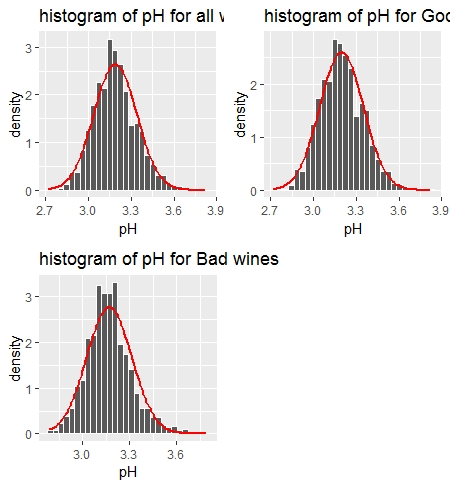
\includegraphics{3_plot_1}
		\end{center}
		\caption{Histograms of pH for all, Good and Bad wines with the of plot a normal density }
	\end{figure}
	
	\begin{figure}[H]
		\begin{center}
			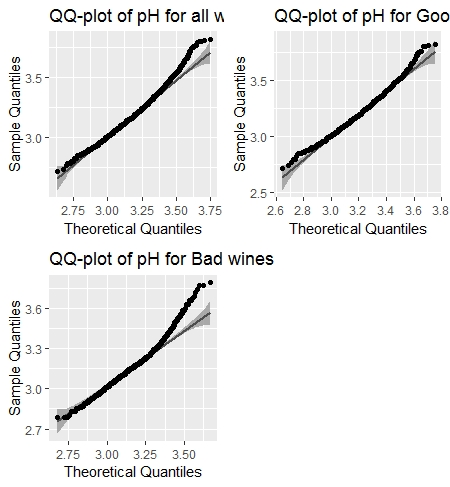
\includegraphics{3_plot_2}
		\end{center}
		\caption{QQ-plots of pH for all, Good and Bad wines}
	\end{figure}

    \begin{figure}[H]
    	\begin{center}
    		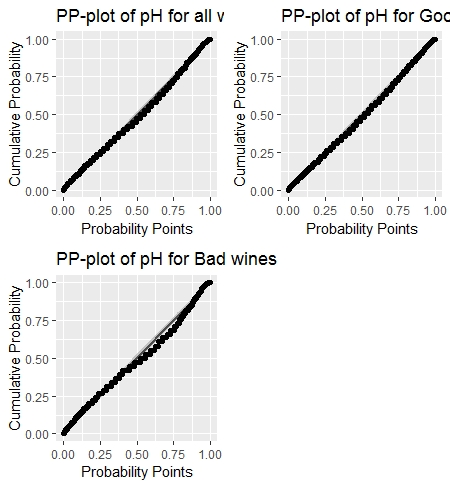
\includegraphics{3_plot_3}
    	\end{center}
    	\caption{PP-plots of pH for all, Good and Bad wines }
    \end{figure}

    \item 
    
    \begin{figure}[H]
    	\begin{center}
    		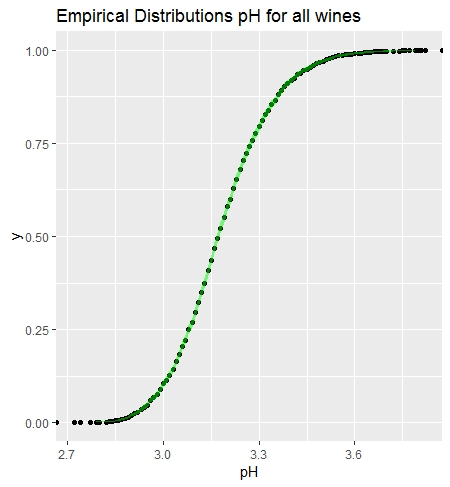
\includegraphics{3_plot_4}
    	\end{center}
    	\caption{Plot of the empirical distribution functions $F_n$ for all three datasets with the pointwise confidence bands for $\alpha = 0.05$}
    \end{figure}

    \begin{figure}[H]
    	\begin{center}
    		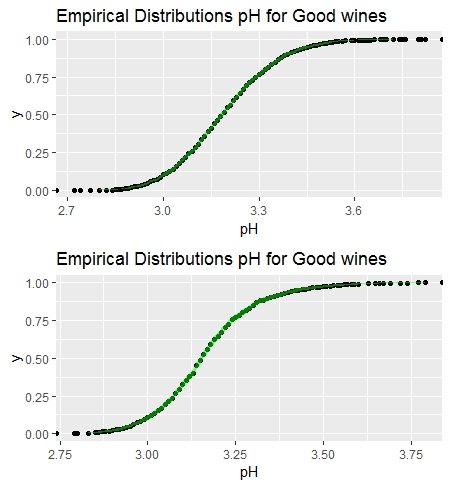
\includegraphics{3_plot_5}
    	\end{center}
    	\caption{Plot of the empirical distribution functions $F_n$ for Good and Bad datasets with the pointwise confidence bands for $\alpha = 0.05$}
    \end{figure}

\end{enumerate}

\chapter{Maximum Likelihood estimation}
The \textbf{maximum likelihood estimation} is a method of estimating the parameters of a statistical model, given observations. It attempts to find the parameter values that maximize the likelihood function, given the observations. The resulting estimate is called a maximum likelihood estimate, which is also abbreviated as MLE.
\section{Introduction and description of the problem}
Let $x_1, x_2,. . . , x_n$  be independent realizations of a r.v. X with
the density function $f (x; \theta), x \in \mathbb{R}, \theta \in \Theta \subset \mathbb{R}^p$. Then, \\
\begin{equation}  %no need to use in this environment $ and $$ are not needed nor allowed in its contents.
\mathcal{L}_x(\theta) =
\prod_{i=1}^{n} f (x_i; \theta)
\end{equation}
is called the \textbf{likelihood function} and \\
\[\widehat{\theta} = \argmax_{\theta \in \Theta} \mathcal{L}_x(\theta) = \argmax_{\theta \in \Theta} \prod_{i=1}^{n} f (x_i; \theta)\]
is the \textbf{maximum likelihood estimate} for $\theta$. \\
Here are some remarks that will be well explained in the following exercise:
\begin{itemize}
	\item Often it is easier to maximize the log-likelihood $\ell$($\theta$) = ln $\mathcal{L}$($\theta$) instead of the likelihood
	L. Since the logarithmic function y = ln(x) is a monotone transformation,
	the solutions to both problems are the same.
	\item MLEs do not always exist (for instance, sometimes the likelihood has a vertical
	asymptote), and even when they do exist, they are not always unique.
	\item  In practice, likelihood functions are sometimes nasty in
	which case we are obliged to use numerical methods to find maxima (if there are
	any).

\end{itemize}

\section{Exercise}
In this exercise, let $X$ be Laplace distributed with parameters $(�; \sigma)^t \in \mathbb{R}�(0; \infty)$, i.e., $X$ has a density: \\
\begin{equation}
f(x) = \frac{1}{2\sigma}\exp(-\frac{|x-�|}{\sigma})
\end{equation}
\begin{enumerate}[label=(\alph*)]
	\item We want to prove that the maximum likelihood estimator for $�$ is the median of the sample
	$(X_1,..., X_n)$ and unique.\\
	Consider the likelihood function for $N$ data samples:
	\begin{equation}
	\mathcal{L}_x(�, \sigma; x)=
	\prod_{t=1}^{N} \frac{1}{2\sigma}\exp(-\frac{|x_t-�|}{\sigma}) = 
	(2\sigma)^{-N} \exp(-\frac{1}{\sigma}\sum_{t=1}^{N}|x_t-�|)
	\end{equation}
	Take the log likelihood funtion, and we get
	\begin{equation}
	\ell_x(�, \sigma; x)=-N\log2\sigma -\frac{1}{\sigma}\sum_{t=1}^{N}|x_t-�|
	\end{equation}
	\begin{equation}
	\frac{\partial\ell}{\partial�}= -\frac{1}{\sigma}\sum_{t=1}^{N} \frac{\partial|x_t-�|}{\partial �}
	\end{equation}
	then we have
	\begin{equation}
	\frac{\partial\ell}{\partial�}= \frac{1}{\sigma}\sum_{t=1}^{N} sgn(x_t-�)
	\end{equation}
	using the identity
	\begin{equation}
	\frac{\partial |x|}{\partial x}= \frac{\partial\sqrt{x^2}}{\partial x}= x(x^2)^{-\frac{1}{2}}= \frac{x}{|x|}= sgn(x)
	\end{equation}
	To maximize the likelihood function we need to solve
	\begin{equation}
	\frac{\partial\ell}{\partial�}=0
	\end{equation}
	For which we have two cases: $N$ is even or odd.\\
	If $N$ is odd and we choose $\widehat{\mu}$ =median$(x_1,...,x_N)$, then there are (N-1)/2 cases where $x_t<\mu$ and for the other (N-1)/2 cases $x_t>\mu$, therefore $\widehat{\mu}$ satisfies (4.8) and is the Maximum likelihood estimator for the parameter $\mu$.\\
	If $N$ is even, we cannot simply choose one $x_t$ which will satisfy (4.8), however we can still minimize it through ranking the observations as $x_1\leq x_2\leq,...,\leq x_N$ and then choosing either $x_\frac{N}{2}$ or $x_\frac{N+1}{2}$.\\
	In summary $\widehat{\mu}$=median$(x_1,...,x_N)$ is the maximum likelihood estimator for any $N$.
	
	\item Now, we generate $n = 20$ independent realisations of $X$ with $\mu = 1$ and $\sigma = 1$, and Determine the maximum likelihood estimator of $\mu$ based on this sample using \textbf{R} function quantile. Actually, According to question (a), the maximum likelihood estimator for mean is the median of the sample $X$. After experimenting the 9 types of sample quantiles in \textbf{R}, types 2, 5, 6, 7, 8 and 9 are most suitable since we have a maximum value of 0.7516658 (which is close to 1) using them.\\
	Then, the sample is increased to $n = 1000$ and we notice that the second median estimator(still with types 2, 5, 6, 7, 8 and 9) gives a result of 0.9767657 which is closer to 1 than 0.7516658.\\
	As result, we can say that the maximum likelihood estimator is more accurate when the sample is enlarged.
	
	\item \item[�] Here, we want to find the maximum likelihood estimator numerically, and we do that by writing the likelihood function and maximise it with the use of \textbf{R} function \textbf{optimise}.\\
	\item[�]The \textbf{optimise} function by default minimizes a function, so we have to set \textbf{maximum = TRUE} to get an MLE. But in the code, we did not need \textbf{maximum = TRUE} because we minimized the negative log-likelihood. The result is 0.7412317 which is close to 0.7516658.\\
	\item[�]For this problem, we cannot employ a Newton-Raphson algorithm because the likelihood function is not twice differentiable.
	\item[�]We generate $n = 20$, $n = 1000$ independent realisations of $X$ with $\mu = 1$ and $\sigma = 1$, and Determine the maximum likelihood estimator of $\mu$ based on these samples using \textbf{R} function \textbf{quantile} and with our function. We can notice that with the \textbf{quantile} function, the suitable types are different. Actually, for the first sample, types 2, 5, 6, 7, 8 and 9 are most fitting for a result of 0.4694639, while for the second sample, types 1, 3, and 4 are most appropriate for a result of 1.023436. With our function, we obtain a result of 0.5285091 for the first sample, and 1.023832 for the second sample.\\
	Overall, the estimators with the second sample, are more accurate (closer to 1) than the one of the first sample. This is probably because the second sample is much larger than the second one. Nevertheless, in both samples, using the \textbf{optimize} function gives a better result than using the \textbf{quantile}. Therefore, in order to have a result closer to 1, we can increase the size of our sample and make use of the \textbf{optimize} function.
	\item Now we study the distribution of the MLE. For this we calculate $M = 5000$ MLEs of $\mu$ based on the samples of n = 20 and n = 1000 random variables generated from the Laplace distribution with $\mu = 1$ and $\sigma = 1$. Repeat the same for the sample size n = 1000.\\
	By looking at the plots in figure 4.1, we can say that our Monte Carlo samples follow a normal distribution, but the approximation of the second sample (n = 1000) is more accurate than the one of the first sample(n =20). Actually, this comes from the fact that on the qq plot of the second sample, points fall on the identity line which indicates a good approximation, while on the other one, the tails are larger than expected (below the line on the left side of the plot and above the line on the right side of the plot). This can be explain by size of the sample, which is larger in the first sample(hence good approximation). This is confirmed with the table below, where the mean and the satandard deviation of the second sample are respectively closer to 1 and 0 than the ones of the first sample.
	
	\begin{center}
		\begin{tabular}{|c|c|c|}
			\hline
			& n = 20 & n = 1000 \\ 
			\hline
			$\mu$ & 0.9911246 & 1.00015424 \\
			\hline
			$sd$ & 0.2615219 & 0.03227411 \\
			\hline
		\end{tabular}
	\end{center}
	
	\begin{figure}[hb]
		\begin{center}
			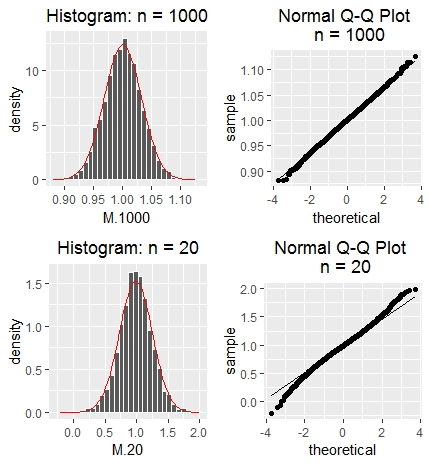
\includegraphics{4_plots.jpeg}
		\end{center}
		\caption{Histograms and qq plots}
	\end{figure}
		
\end{enumerate}



\chapter{Tests for categorical data }
\section{Introduction and description of the problem}
In this section, in order to analyze dependencies and homogeneity in a data, we will make use of the folling tests: the Binomial test, the exact Fisher test, and the $\chi^2$-test. \\

\section{Exercise}

All tests to the significance level $\alpha = 0.05$. The dataset is the above table, representing the delayed flights from Exercise 1.
\begin{center}
	\begin{tabular}{|c|c|c|}
		\hline
		& Alaska.Airlines.Delayed  & America.West.Delayed \\ 
		\hline
		Los Angeles & 62 & 117 \\
		\hline
		Phoenix & 12 & 415 \\
		\hline
		San Diego & 20 & 65 \\
		\hline
		San Francisco & 102 & 129 \\
		\hline
		Seattle & 305 & 61 \\
		\hline
	\end{tabular}
\end{center}

\begin{enumerate}[label=(\alph*)]
	\item In order to to test if the delay is independent on the city for each airline, can make use of the test statistics $\chi^2 = \sum_{i=1}^{12}\frac{(O_i - E_i)^2}{E_i} \overset{approx}{\sim} \chi^2_4 $ , where 4 is the degree of freedom, $O_i$ and $E_i$ are respectively the observed and expected (under $H_0$: indepence between the delays in each city) frequencies.\\
	When we run this on R,  obtain a value of 550.5328. Then we the help of the Chi-square distribution table, we have a p-value $ = \mathtt{P}(\chi^2_4 > 550.5328) \ll \alpha $. Therefore we accept $H_0$, that is the delay is independent on the city for each airline.\\
	This is confirmed when running the command $\mathbf{chisq.test}$, since we obtain a $p-value < 2.2*10^{-16}$\\
	
	\item Here, we want to check if the delay is independent on the airline. For that, we find first the total delays in each airline (see the table below), and we run the Chi-square test.\\
	\begin{center}
		\begin{tabular}{|c|c|c|}
			\hline
			& Alaska.Airlines.Delayed & America.West.Delayed \\ 
			\hline
			Total.Delayed & 501 & 787 \\
			\hline
		\end{tabular}
	\end{center}
	We obtain a p-value $ = 1.599*10^{-15} < \alpha$, that is the delay is independent on the airline.
	
	\item In order to test for each airline, if the delay probability equals to 0.14, we make use of the binomial test under $H_0$ : the delay probability equals 0.14 . In each airline, we can consider the number of delays as successes, and on time as failures. The test gives us the following p-values, 0.2053 and $3.898*10^{-15}$ repectively for $\mathbf{Alaska.Airlines.Delayed}$ and $\mathbf{America.West.Delayed}$. Therefore, at the significance level of $\alpha = 0.05$, we conlcude that the delay probability equals to 0.14 for $\mathbf{Alaska.Airlines.Delayed}$, while it is not the case for $\mathbf{America.West.Delayed}$.\\
	Then, when performing the one-sided alternative that the delay probability is larger than 0.14, we obtain p-value of 0.9062 for $\mathbf{Alaska.Airlines.Delayed}$ and 1 for $\mathbf{America.West.Delayed}$. What cahnges in this case is that we accept $H_0$ :  the d$\alpha$lay probability is larger than 0.14, since both p-values are greater than $\alpha$.
\end{enumerate}

\chapter{Tests for quantitative data}
\section{Introduction and description of the problem}
In this section, we want to make use of Wilcoxon test, unpaired and paired t-test, in order to compare to independent samples.

\section{Exercise}
For this exercise, we use the data on US 2016 presidential race.

\begin{enumerate}[label=(\alph*)]
	\item For this question, we add a new binary variable $ \mathbf{vote} $, which assigns 1 if the
	majority in the county voted for Clinton and 0 if the majority voted for Trump. Then we divide variable $ \mathbf{Diversity.Index} $ into two groups: the one that corresponds to 1 in vote and another one that corresponds to 0 in vote. \\
	By looking at figure 6.1, we can assume that the diversity index in the group with vote = 1 is normally distributed, while it is not for the group with vote = 0. Actually, this is a direct intepretation of the histograms and qq-plots. The points on the qq-plot of the Diversity index for vote = 1 are close to the line, which means that the distribution is close to normal. In contrast, the points for the Diversity index with vote = 0 are far away from the line, especially on the left, indicating that the distribution is skewed. We have the same results using histograms.
	
	\begin{figure}[H]
		\begin{center}
			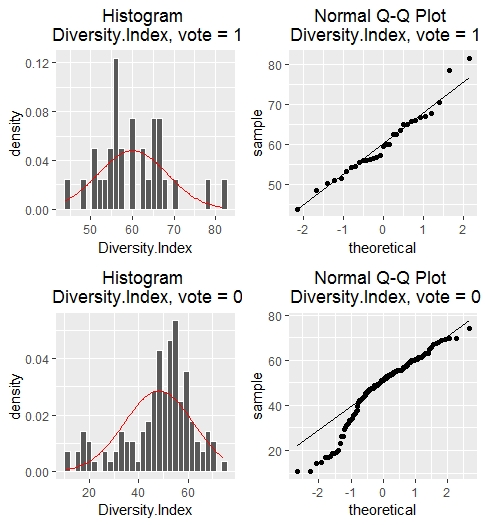
\includegraphics{6_plot_1.jpeg}
		\end{center}
		\caption{Histograms and qq-plots for Diversity.Index with vote = 0 and 1}
	\end{figure}

    \item Here, we want to test at the significance level $\alpha = 0.05$, if the diversity index in the group that voted for Clinton is significantly larger than that in the group that voted for Trump.
    
     \item[�] According to question (a), since no normality has been assumed for one of the group, one rather tests under $H_0$: both groups have the same median. We need to test beforehand the independence between the two groups. With the Chi-square test, we have a p-value $< 2.2*10^{-16}$, that is the independence assumtion is verified. Now we use the t-test. Note that we do not need to check weather or not the two groups have the same variance.\\
     For the t-test, we have a p-value $= 3.035*10^{-08} < \alpha$, hence we accept $H_0$, that is both groups have the same median at a significance level of 0.05 . 
     
    
      \item[�] With a wilcoxon-test, we have the same conclusion as the p-value $= 3.72*10^{-06} < \alpha$
          
      \item By looking at figure 6.2, we can assume that diversity index for both groups is not normally distributed. Actually, The points on the lower left side of the qq-plot of Diversity.index are not matching the horizontal line, which means that the distribution is not normal. This is confirmed with the histogram which skewed to the left.
      
       \begin{figure}[H]
       	\begin{center}
       		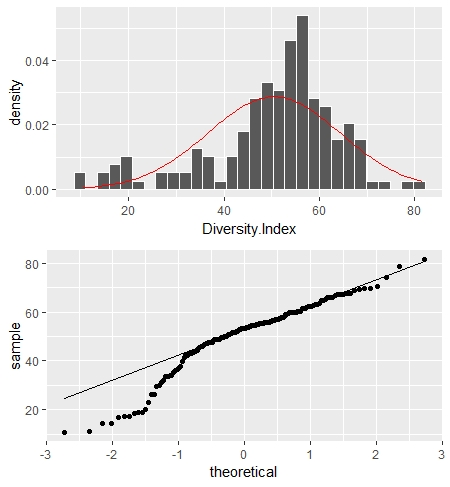
\includegraphics{6_plot_2.jpeg}
       	\end{center}
       	\caption{Histograms and qq-plots for Diversity.Index}
       \end{figure}
	
	\item [�] When we run the t-test, we have a p-value $= 2.2 \times 10^{-16} < \alpha$, and the same for the Wilcoxon-test. This can be explained by the fact Diversity.Index is not normally distributed, which is the most important property to run these tests. Actually, their outcome is to estimate the mean of a normally distributed dataset. If the dataset is not normally distributed, we can rather estimate the median. 
	
\end{enumerate}

\chapter{Linear regression}
\section{Introduction and description of the problem}
In this section we explore linear regression, which is a linear approach to modelling the relationship between a scalar response (or dependent variable) and one or more explanatory variables (or independent variables). The case of one explanatory variable is called simple linear regression. For more than one explanatory variable, the process is called multiple linear regression.

\section{Exercise}
In this ecercise, we want to achieve the two main goals of linear regression which are prediction/forecasting/ error reduction and explaination of variation in the response variabl. For that, we use the dataset on house prices from Kaggle.com, which contains house sale prices for King County, which includes Seattle.

\begin{enumerate}[label=(\alph*)]
	\item We want to estimate a linear model with the response variable price and all remaining variables as covariates.
	\item[�] The p-value of all variables is less than 0.05, which means that all variables are significant.
	\item[�] The $R^2 = 0.6359$ of our model indicates that the model explains more than half ( about $63\%$) of the variability of the response data around its mean.
	\item[�] $\mathbf{Residual Analysis}$\\
	Normality Assumption: If the assumption of normality were true, then we would expect points randomly scattered about the dotted straight line displayed in the figure4.1 . In this case, we see thatThe points on the lower left and upper right of the plot stray from the line. We would say
	that the residuals are not normal.
	
		\begin{figure}[H]
		\begin{center}
			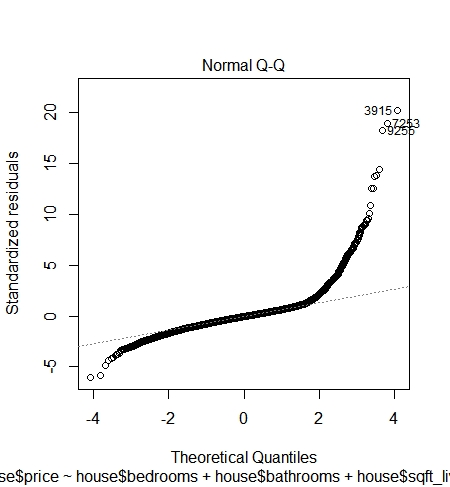
\includegraphics{7_plot_1}
		\end{center}
		\caption{A qq-plot of the residuals from the linear regression model in (a) }
	\end{figure}
	
	Constant Variance Assumption: When we look at Figure 7.2, we can notice a fanning-out of the dots, of the residuals. This patterns indicate a change in the residual variance and a consequent
	departure from the regression assumptions, an increase in this case.
	
	\begin{figure}[H]
		\begin{center}
			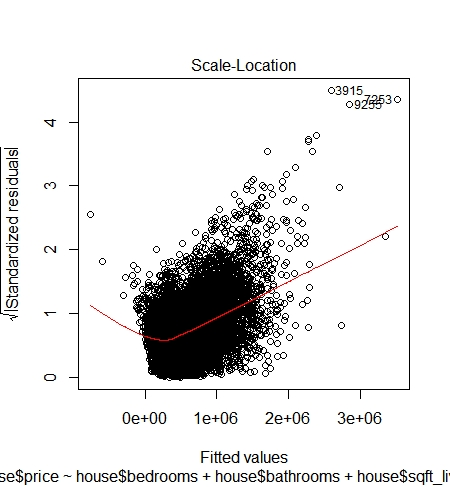
\includegraphics{7_plot_2}
		\end{center}
		\caption{Plot of the standardized residuals versus the fitted values}
	\end{figure}

	Independence Assumption: from Figure 7.3, we can notice that the points form a cone-like shape indecating a problem of Heteroskedasticity.
	
	\begin{figure}[H]
		\begin{center}
			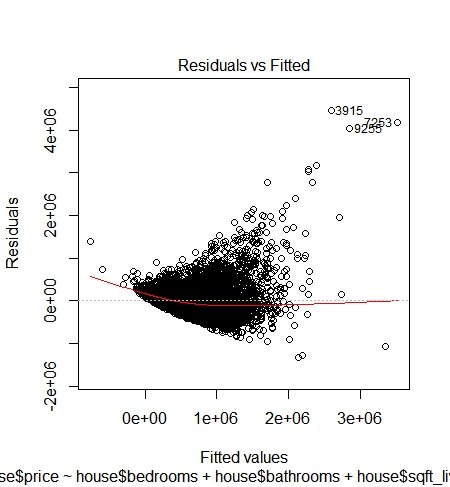
\includegraphics{7_plot_3}
		\end{center}
		\caption{Plot of the residuals versus the fitted values}
	\end{figure} 
	
	\item \item[�] Compared to a normal distribution, log(price) is much likely to follow a normal distribution than the variable price. Actually, from Figure 7.4, we notice from the bins on the price variable histogram are more represented in the left than those of the logprice variable: the skewness' coefficient (in absolute value) price is greater than the one log(price). Furthermore, the q-q plot of the variable price highlights points that are much fanning-out at the upper end of the graph, than those of the q-q plot logprice variable.
	
	\begin{figure}[H]
		\begin{center}
			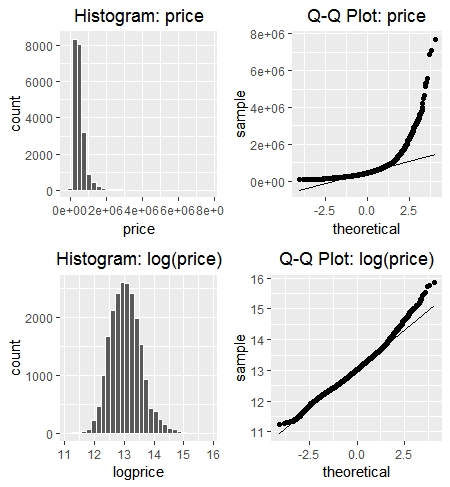
\includegraphics{7_plot_4}
		\end{center}
		\caption{Histograms and qq-plot for price and log(price)}
	\end{figure}

    \item[�] Now a linear model is fitted with the response variable log(price). Compared to the previous model, all coefficients are significant(since the p-value $<0.05$ ). Nevertheless, $R^2 = 0.6426$ is greater than the 0.6359 that we had before. This suggest that the second model is better than the first one. This can be confirmed with the following residual analysis:\\
    In Figure 7.5, the q-q plot suggest that the residuals follow a normal distribution as all points are a long the straight line. Then, the fitted values plot shows the points randomly scattered on the plot, which means that there is very little evidence of nonzero autocorrelation in the residuals. Finally, the plot of standardized residuals against the fitted values, even though there is arguably no constant band of observations, the deplacement of points suggest that the variance is more likely to be constant in this model than in the previous one.
    
    \begin{figure}[H]
    	\begin{center}
    		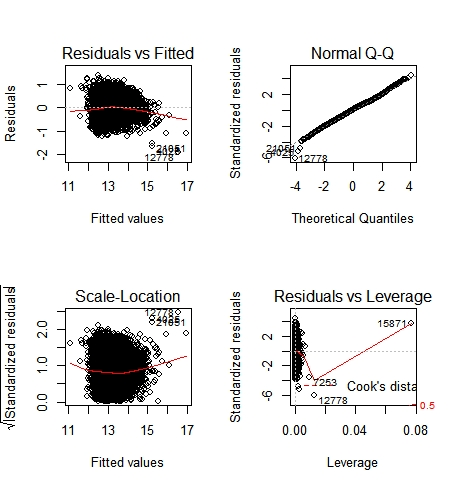
\includegraphics{7_plot_5}
    	\end{center}
    	\caption{Plots for the second model's residual analysis log(price)}
    \end{figure}
    
    \item \item [�] From the second model(the one from (b)), we have the following interpretation of the covariates: for 1$\%$ of bathrooms, sqft\_living, floors, view, condition, and grade will have a positif effect on the response variables with the following proportions respectively 8.49\%,      0.01$\%$, 08.56$\%$, 6.73$\%$, 4.22$\%$, and 22.17$\%$, while for 1\% of bedrooms and yr\_built, we will have a negatif effect respectively with the following proportions 2.36\%, and 0.55\%.
    \item [�] From the following Figure 7.6, it is trivial that the assumption of the linear dependence between
    covariates and response is not plausible for all covariates.
    
    \begin{figure}[H]
    	\begin{center}
    		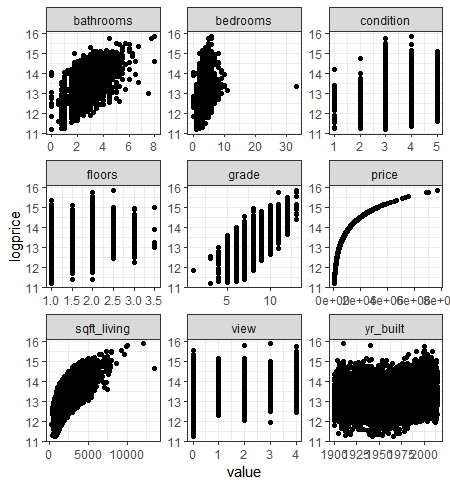
\includegraphics{7_plot_6}
    	\end{center}
    	\caption{Plots of each covariate against log(price)}
    \end{figure}
    
    \item [�] After adding to the first model squared terms for yr\_built and sqft\_living, we notice that they are significant since the p-value $<0.05$ . Furthermore, these two terms improve the model fit in terms of $R^2$, which is 0.6681 > 0.6426 .
    
    \item Now we would like to compare how well models from (b) and (c) make prediction. For this we divide the dataset into a training and a test set. Then we fit both models on the training set
    and make prediction on the test set. 
    \item[�] The mean squared difference between predicted values and values of log(price) from the test set for the model in (b) is 0.1003765, while we have 0.0985067 for the model in (c). The model from (c) has the smallest error. In order to improve the prediction, the squared term on yr\_built has been changed to the power of 10, and we a get an error of 0.09653776.
    
\end{enumerate}

\chapter{Logistic regression }
\section{Introduction and description of the problem}

We now look at another form of regression, the logistic regression. Sometimes the dependence cannot be described with a linear model so we sometimes have to use other models, e.g. the logit-model. There are also some missing assumptions like normal distributed errors and homoscedacity. The logistic regression can be seen as a special case of the generalized linear model.

\section{Exercise}
In this exercise, we use the dataset from UCI Machine learning repository on blood donation. The goal is to build a model that allows to predict best if a donor will donate the blood.

\begin{enumerate}[label=(\alph*)]
	\item Here, we have one model GLM.1 which is a fit a generalised linear model fitted with the binary response donation and covariate frequency (using the canonical link function),  and another model GLM.2 which fits the same model by replacing the covariate by amount.
	\item[�] When we run the summary of the second model(GLM.2), we almost have the same results as in the first one.
	\item[�] When we plot variable frequency against amount as shown in Figure 8.1, points fall exactly on the identity line; using these variables into a moddel would be like using one of them twice. Therefor, we do not need both of them into the model.
	
	\begin{figure}[H]
		\begin{center}
			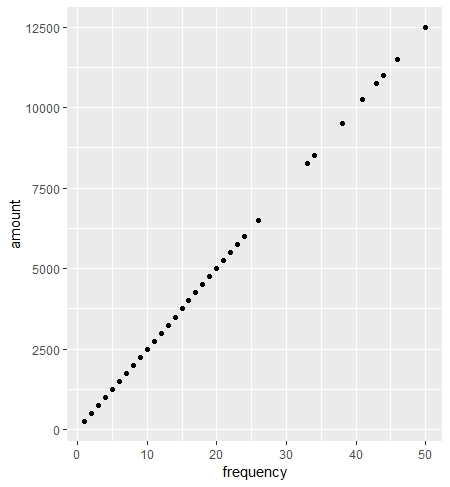
\includegraphics{8_plot_1}
		\end{center}
		\caption{Plot variable frequency against amount}
	\end{figure}
	
	\item \item[�] Now, after fitting the the GLM model with the response donation and covariate recency using
	all link functions available in the glm function, we obtain five models: GLM.3(with logistic CDF), GLM.4(with normal CDF), GlM.5(with Cauchy CDF), GLM.6(with logarithm CDF) and GLM.7(with complementary log-log). The following table highlights the AIC of the models, and we notice that the GlM.7 has the lowest AIC, then this model is more parsimonious according to the AIC.
	
	\begin{center}
		\begin{tabular}{|c|c|c|c|c|c|}
			\hline
			& GLM.3 & GLM.4 & GLM.5 & GLM.6 & GLM.7\\ 
			\hline
			AIC & 747.5547 & 748.3307 & 749.4959 & 747.6188 & 747.4671 \\
			\hline
		\end{tabular}
	\end{center}

	\item[�] In order to chose between all links, we use the Figure 8.2. From that graph, we can choose cauchit as our best link function, because for the others, after 60 months, the functions tend to zero meaning that there is no more blood donation after this period which is weird.
	
	\begin{figure}[H]
		\begin{center}
			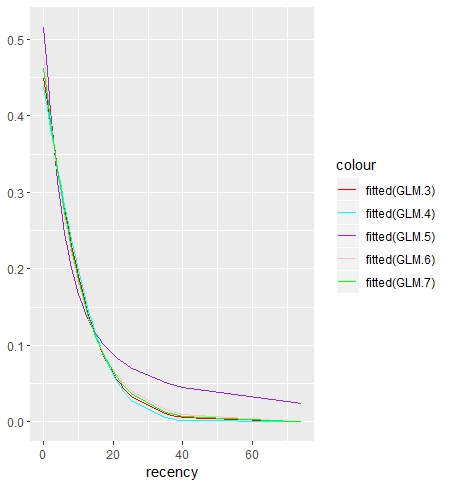
\includegraphics{8_plot_2}
		\end{center}
		\caption{reponse variable recency against fitted of each model}
	\end{figure}
	
	\item Now we fit a model called GLM.8 with the response variable donation and the canonical link that makes the best prediction for the blood donations. By choosing appropriate covariates, we predict the model on a test set. The Figure 8.3 we can suggest that frequency or amount can give us a good prediction model.\\
	
	\begin{figure}[H]
		\begin{center}
			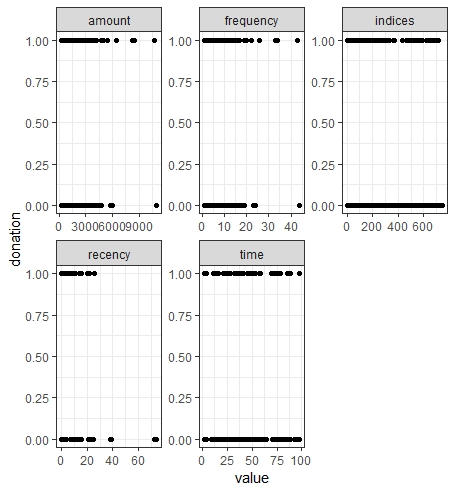
\includegraphics{8_plot_3}
		\end{center}
		\caption{Plots of each covariate against donation}
	\end{figure}
	
	After performing the prediction, we use the predicted probability to perform the following classification: the predicted $i^{th}$ value of donation to 0, when the corresponding $i^{th}$ predicted probability is less than 0.5 and to 1 otherwise. Now we can assess the goodness of our classification, with the classification error:
	
	\begin{equation}
	CE= \frac{1}{374}\sum_{i=1}^{374} |y^{test}_i-\widehat{y}^{test}_i|
	\end{equation}
	
	Where $y^{test}_i$ is the ith value of donation from the test set and $y^{test}_i$ is its prediction.\\
	With the covariate frequency, the CE of 0.2085561 has been beaten to 0.197861. We have the same reult with amount.
	
\end{enumerate}

\chapter{Penalised regression}

\section{Introduction and description of the problem}
In this section, we will use two penalised regressions, Ridge and Lasso. Ridge Regression is a technique for analyzing multiple regression data that suffer from multicollinearity(  existence of near-linear relationships among the independent variables). Multicollinearity can create inaccurate estimates of the regression coefficients, inflate the standard errors of the
regression coefficients, deflate the partial t-tests for the regression coefficients, give false, nonsignificant, pvalues, and degrade the predictability of the model When multicollinearity occurs, least squares estimates are unbiased, but their variances are large so they may be far from the true value. By adding a degree of bias to the regression estimates, ridge regression reduces the standard errors. It is hoped that the net effect will be to give estimates that are more reliable.\\
Lasso is another technique for analysis that performs both variable selection and regularization in order to enhance the prediction accuracy and interpretability of the statistical model it produces.

\section{Exercise}

In this exercise, we consider the dataset hitters.dat on baseball players that has been analysed in the book \textit{An introduction to statistical learning by G. James, D. Witten, T. Hastie and R. Tibshirani} (2013, Springer). 

\begin{enumerate}[label=(\alph*)]
	\item Cf. the R code
	
	\item \item[�] The condition number of $X^tX$, where $y$ is the salary and $X$ represents all the other  variables, is given by 558855577. This large condition number indicate multicollinearity.
	\item[�] By  standardising the design matrix, such that its columns (without the intercept) have mean zero and variance one, we obtain a condition value of 5019.26, way less than the previous one. Thus it helps the standardisation of the design matrix.
	
	\item After fitting a standard linear model (no regularisation) and a ridge regression with $\lambda = 70$, we observe that the coefficients (in absolute value ) of the linear model are larger the ones of the ridge regression.
	\item The value 70 for $\lambda$ is arbitrary and we would like to find a data-driven way to choose
	it. The criterion to compare is the mean squared prediction error as in exercise 7(d)
	on linear regression. Cf. R code
	\item From Figure 9.1, the $\lambda_{opt}$ that minimises the mean squared prediction error (MSE) can be $10^2$.
	
	\begin{figure}[H]
		\begin{center}
			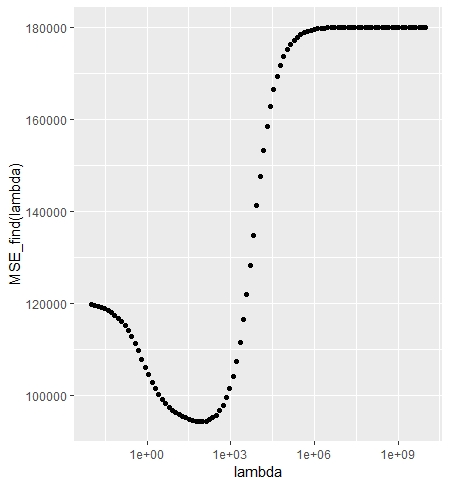
\includegraphics{9_plot_1}
		\end{center}
		\caption{Ridge: log($\lambda$) against the MSE}
	\end{figure}
	
	\item Now, we fit a ridge regression with $\lambda_{opt}$ on all the data. Since we are running a penalised regression, we notice that all coefficients are shrinking to 0, except the ones for League and Divion ( 36.77 and -108.67 respectively), thus they are less important in the prediction, and League and Divion are the most important variables. Despite the use of $\lambda_{opt}$, there is no coefficient exactly equal to 0.\\
	
	\item We repeat Repeat (e), (f) for Lasso.
	\item[(e')] From Figure 9.2, the $\lambda_{opt}$ that minimises the mean squared prediction error (MSE) can be $10^{1.4}$.
	
	\begin{figure}[H]
		\begin{center}
			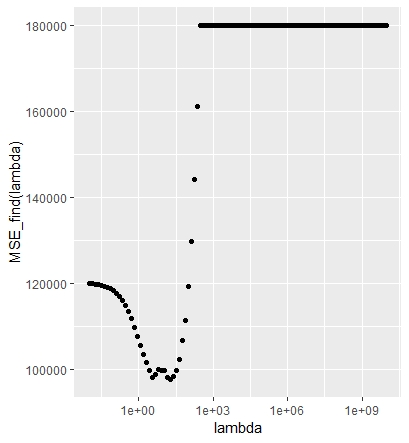
\includegraphics{9_plot_2}
		\end{center}
		\caption{Lasso: log($\lambda$) against the MSE}
	\end{figure}

    \item[(f')] Now, we fit a Lasso regression with the new $\lambda_{opt}$ on all the data. Now, we notice that coefficients of some variables, that are: Assists, Errors, NewLeague, CWalks, League, Years, CAtBat, CHits, CHmRun, AtBat, HmRun, Runs, RBI, are exactly equal to 0.

\end{enumerate}

\chapter{Principal component analysis}
In this part, we want to use Principal component analysis (PCA) in order to summarize the information in a data set described by multiple variables.

\section{Introduction and description of the problem}
PCA is defined as an orthogonal linear transformation that transforms the data to a new coordinate system such that the greatest variance by some projection of the data comes to lie on the first coordinate (called the first principal component), the second greatest variance on the second coordinate, and so on. \\
Let $ X \in \mathbb{R}^{n \times p} $ be a matrix that contains $n$ observations of $p$ variables.\\
Denote $ \bar{X} = n^{-1}\sum_{j=1}^{n} X_{ij} $ , the sample mean of the $i^{th}$ column of $X$
and $ \tilde{X} = X -(\bar{X}_{1} \mathnormal{1}_n,...,\bar{X}_{n} \mathnormal{1}_n) $ for $ {1}_n = (1,...,1)^t $ the centered matrix.\\
From the eigenvalue decomposition $ \tilde{X}^t\tilde{X} = Udiag(\lambda_{1},...,\lambda_{p}))U^t $. one finds scores $\lambda_i$, loadings $U_i$ ($i^{th}$ column), principal components $ P = \tilde{X}U \in \mathbb{R}^{n \times p} $. The $i^{th}$ column of $P$ is called the $i^{th}$ principal components.

\section{Exercise}

In this section, we use the dataset \textbf{iris} which is a classical dataset in statistics. It contains five variables all measured in centimeters.

\begin{enumerate}[label=(\alph*)]
	\item From the the table below, we notice that PC1 and PC2 account for respectively, 92.46\% and 5.3\% of the total variation in the data. Therefore, PC1 explains much more of the variability in the data than PC2, and we will have to retain PC1.
	
	\begin{center}
		\begin{tabular}{|c|c|c|c|c|}
			\hline
			        & PC1  &   PC2  &  PC3  &   PC4\\ 
			\hline
			Standard deviation  &   2.0563 & 0.49262 & 0.2797 & 0.15439 \\
			\hline
			Proportion of Variance & 0.9246 & 0.05307 & 0.0171 & 0.00521 \\
			\hline
			Cumulative Proportion & 0.9246 & 0.97769 & 0.9948 & 1.00000 \\
			\hline
		\end{tabular}
	\end{center}

\begin{center}
	\begin{tabular}{|c|c|c|c|c|}
		\hline
		& PC1  &   PC2  &  PC3  &   PC4\\ 
		\hline
		Sepal.Length & 0.36138659 & -0.65658877 &  0.58202985 & 0.3154872 \\
		\hline
		Sepal.Width & -0.08452251 & -0.73016143 & -0.59791083 & -0.3197231 \\
		\hline
		Petal.Length & 0.85667061 & 0.17337266 & -0.07623608 & -0.4798390 \\
		\hline
		Petal.Width & 0.35828920 & 0.07548102 & -0.54583143 & 0.7536574 \\
		\hline
	\end{tabular}
\end{center}
	
	\item The two tables below are the loadings and scores when we use the empirical correlation matrix. We observe that the results are different. For exemple, compared to the previous one, PC1 still explains more of the variability in the data than PC2, but with a proportion of 72.96\%.
	
	\begin{center}
		\begin{tabular}{|c|c|c|c|c|}
			\hline
			& PC1  &   PC2  &  PC3  &   PC4\\ 
			\hline
			Standard deviation  &  1.7084 & 0.9560 & 0.38309 & 0.14393 \\
			\hline
			Proportion of Variance & 0.7296 & 0.2285 & 0.03669 & 0.00518 \\
			\hline
			Cumulative Proportion & 0.7296 & 0.9581 & 0.99482 & 1.00000 \\
			\hline
		\end{tabular}
	\end{center}
	
	\begin{center}
		\begin{tabular}{|c|c|c|c|c|}
			\hline
			& PC1  &   PC2  &  PC3  &   PC4\\ 
			\hline
			Sepal.Length & 0.5210659 & -0.37741762 &  0.7195664 &  0.2612863 \\
			\hline
			Sepal.Width & -0.2693474 & -0.92329566 & -0.2443818 & -0.1235096 \\
			\hline
			Petal.Length & 0.5804131 & -0.02449161 & -0.1421264 & -0.8014492 \\
			\hline
			Petal.Width &  0.5648565 & -0.06694199 & -0.6342727 & 0.5235971 \\
			\hline
		\end{tabular}
	\end{center}
    
    \item The two tables below represent respectively, the summary of the dataset (with petal length in millimetres) using the covariance matrix, and the correlation matrix. We notice that results, especially for the proportion of variance explained, has only changed with the covariance matrix.
    
    \begin{center}
    	\begin{tabular}{|c|c|c|c|c|}
    		\hline
    		& PC1  &   PC2  &  PC3  &   PC4\\ 
    		\hline
    		Standard deviation  &  17.6840 & 0.50221 & 0.28081 & 0.1754 \\
    		\hline
    		Proportion of Variance & 0.9988 & 0.00081 & 0.00025 & 0.0001 \\
    		\hline
    		Cumulative Proportion & 0.9988 & 0.99965 & 0.99990 & 1.0000 \\
    		\hline
    	\end{tabular}
    \end{center}
	
	\begin{center}
		\begin{tabular}{|c|c|c|c|c|}
			\hline
			& PC1  &   PC2  &  PC3  &   PC4\\ 
			\hline
			Standard deviation  &  1.7084 & 0.9560 & 0.38309 & 0.14393 \\
			\hline
			Proportion of Variance & 0.7296 & 0.2285 & 0.03669 & 0.00518 \\
			\hline
			Cumulative Proportion & 0.7296 & 0.9581 & 0.99482 & 1.00000 \\
			\hline
		\end{tabular}
	\end{center}
    
    \item From the biplot of the first two principal components against each other(Figure 10.1), \item[�] observe that Petal.Length, Petal.Width, and Sepal.Length have positive loadings on component 1. We can also point out how Species are grouped in three clusters, with two groups of Species, versicolor and virginia, very close.
	\item[�] Interprepreting results from a four-dimensional space is not easy, since we are already used to a twodimensional space. Therefore, it is reasonable to think that we can easily get information out of this plot, than the original four-dimensional space.
	
	\begin{figure}[H]
		\begin{center}
			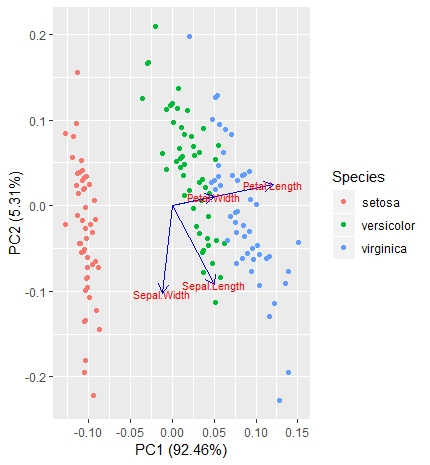
\includegraphics{10_plot_1}
		\end{center}
		\caption{Plot the first two principal components against each other}
	\end{figure}

    \item After performing K-means clustering for the first two principal components obtained in (a)
    with K = 3, we have the table below. We can notice that clusters coincide with the setosa iris species, but it not the case for the other species. This confirms what we noticed previously in Figure 10.1 . The classification error in this case is given by: $\frac{50 + 47 + 36}{50 + 47 + 3 + 14 + 36} = 88.67\%  $
    
    \begin{center}
    	\begin{tabular}{|c|c|c|c|}
    		\hline
    		& setosa & versicolor & virginica \\ 
    		\hline
    		1st Cluster   &   0    &     47    &    14 \\
    		\hline
    		2nd Cluster   &  50    &      0    &     0 \\
    		\hline
    		3rd Cluster   &   0    &     3     &   36 \\
    		\hline
    	\end{tabular}
    \end{center}
    
    The table above correspond to the results of the K-means clustering performed on the whole dataset. The classification error in this case is given by: $\frac{50 + 48 + 36}{50 + 48 + 2 + 14 + 36} = 89.33\% $, which is greater than the one we had previously. This means that using the classification with the first two principal components is better than the classification on the whole dataset.
    
    \begin{center}
    	\begin{tabular}{|c|c|c|c|}
    		\hline
    		& setosa & versicolor & virginica \\ 
    		\hline
    		1st Cluster   &   0    &     48    &    14 \\
    		\hline
    		2nd Cluster   &  50    &      0    &     0 \\
    		\hline
    		3rd Cluster   &   0    &     2     &   36 \\
    		\hline
    	\end{tabular}
    \end{center}
    
	
\end{enumerate}

\end{document}